\chapter{RELATED WORKS}

\renewcommand{\headrulewidth}{0.5pt}
\renewcommand{\footrulewidth}{0.5pt}
\thispagestyle{plain}
\pagestyle{fancy}
\fancyhf{}
\fancyhead[L]{\textbf{CHAPTER 3}}
\fancyhead[R]{\textbf{DANGEGOUS WEAPONS DETECTION USING YOLOv9}}
\raggedright
\fancyfoot[L]{From: Nguyen Van Anh Tuan}
\fancyfoot[R]{Page \thepage}

\justifying

\section{Collect Dataset}
    \subsection{Choose Type of Dataset}
        Nowaday, on market, there are many type of dataset format we can use for training model purpose. For detection, we will have a lot of dataset format like:
        \begin{itemize}
            \item Argoverse
            \item COCO
            \item LVIS
            \item COCO8
            \item GlobalWheat2020
            \item Objects365
            \item OpenImagesV7
            \item SKU-110K
            \item VOC
            \item xView
            \item Roboflow 100
            \item Brain-tumor
            \item African-wildlife 
            \item Signature
        \end{itemize}
        For segmentation, we will have:
        \begin{itemize}
            \item COCO 
            \item COCO8-seg 
            \item Crack-seg 
            \item Carparts-seg 
            \item Package-seg 
        \end{itemize}
        For pose, we will have:
        \begin{itemize}
            \item COCO
            \item COCO8-pose
            \item Tiger-pose
        \end{itemize}
        For classification, we have:
        \begin{itemize}
            \item Caltech 101 
            \item Caltech 256
        \end{itemize}
        In this project, i'll choose COCO dataset work with it.
        \subsubsection{Overview COCO Dataset}
            The \textbf{COCO (Common Objects in Context)} dataset is a large-scale object detection, segmentation, and captioning dataset. It is designed to encourage research on a wide variety of object categories and is commonly used for benchmarking computer vision models. It is an essential dataset for researchers and developers working on object detection, segmentation, and pose estimation tasks.
            \begin{figure}[H]
                \centering
                
\includegraphics[width=0.8\linewidth]{img/coco-logo.png}
                \caption{COCO Dataset}
                \label{fig:coco}
            \end{figure}
        \subsubsection{COCO Pretrained Models}
            \begin{table}[ht]
                \centering
                \begin{adjustbox}{width=\textwidth}
                \small
                \begin{tabular}{| c | c | c | c | c | c | c |}
                    \hline
                    \rowcolor{lightgray} Model & Size (pixels) & mAP${^{val}_{50:95}}$ & Speed CPU ONNX (ms) & Speed A100 TensorRT (ms) & params (M) & FLOPs (B) \\ \hline
                    YOLOv8n & 640 & 37.3 & 80.4 & 0.99 & 3.2 & 8.7 \\ \hline
                    YOLOv8s & 640 & 44.9 & 128.4 & 1.20 & 11.2 & 28.6 \\ \hline
                    YOLOv8m & 640 & 50.2 & 234.7 & 1.83 & 25.9 & 78.9 \\ \hline
                    YOLOv8l & 640 & 52.9 & 375.2 & 2.39 & 43.7 & 165.2 \\ \hline
                    YOLOv8x & 640 & 53.9 & 479.1 & 3.53 & 68.2 & 257.8 \\ \hline
                \end{tabular}
                \end{adjustbox}
                \caption{COCO Pretrained Models}
                \label{tab:coco-pretrained}
            \end{table}
        \subsubsection{Key Feature}
            COCO is a large-scale object detection, segmentation, and captioning dataset. COCO has several features:
            \begin{itemize}
                \item Object segmentation
                \item Recognition in context
                \item Superpixel stuff segmentation
                \item 330K images (>200K labeled)
                \item 1.5 million object instances
                \item 80 object categories
                \item 91 stuff categories
                \item 5 captions per image
                \item 250,000 people with keypoints
            \end{itemize}
        \subsubsection{Data Structure}
            The COCO dataset is split into three subsets:
            \begin{enumerate}
                \item \textbf{Train2017:} This subset contains 118K images for training object detection, segmentation, and captioning models.
                \item \textbf{Val2017:} This subset has 5K images used for validation purposes during model training.
                \item \textbf{Test2017:} This subset consists of 20K images used for testing and benchmarking the trained models. Ground truth annotations for this subset are not publicly available, and the results are submitted to the COCO evaluation server for performance evaluation.
            \end{enumerate}
        \subsubsection{Applications}
            The COCO dataset is widely used for training and evaluating deep learning models in object detection (such as YOLO, Faster R-CNN, and SSD), instance segmentation (such as Mask R-CNN), and keypoint detection (such as OpenPose). The dataset's diverse set of object categories, large number of annotated images, and standardized evaluation metrics make it an essential resource for computer vision researchers and practitioners.
        \subsubsection{Sample Images and Annotations}
            The COCO dataset contains a diverse set of images with various object categories and complex scenes. Here are some examples of images from the dataset, along with their corresponding annotations:
            \begin{figure}[H]
                \centering
                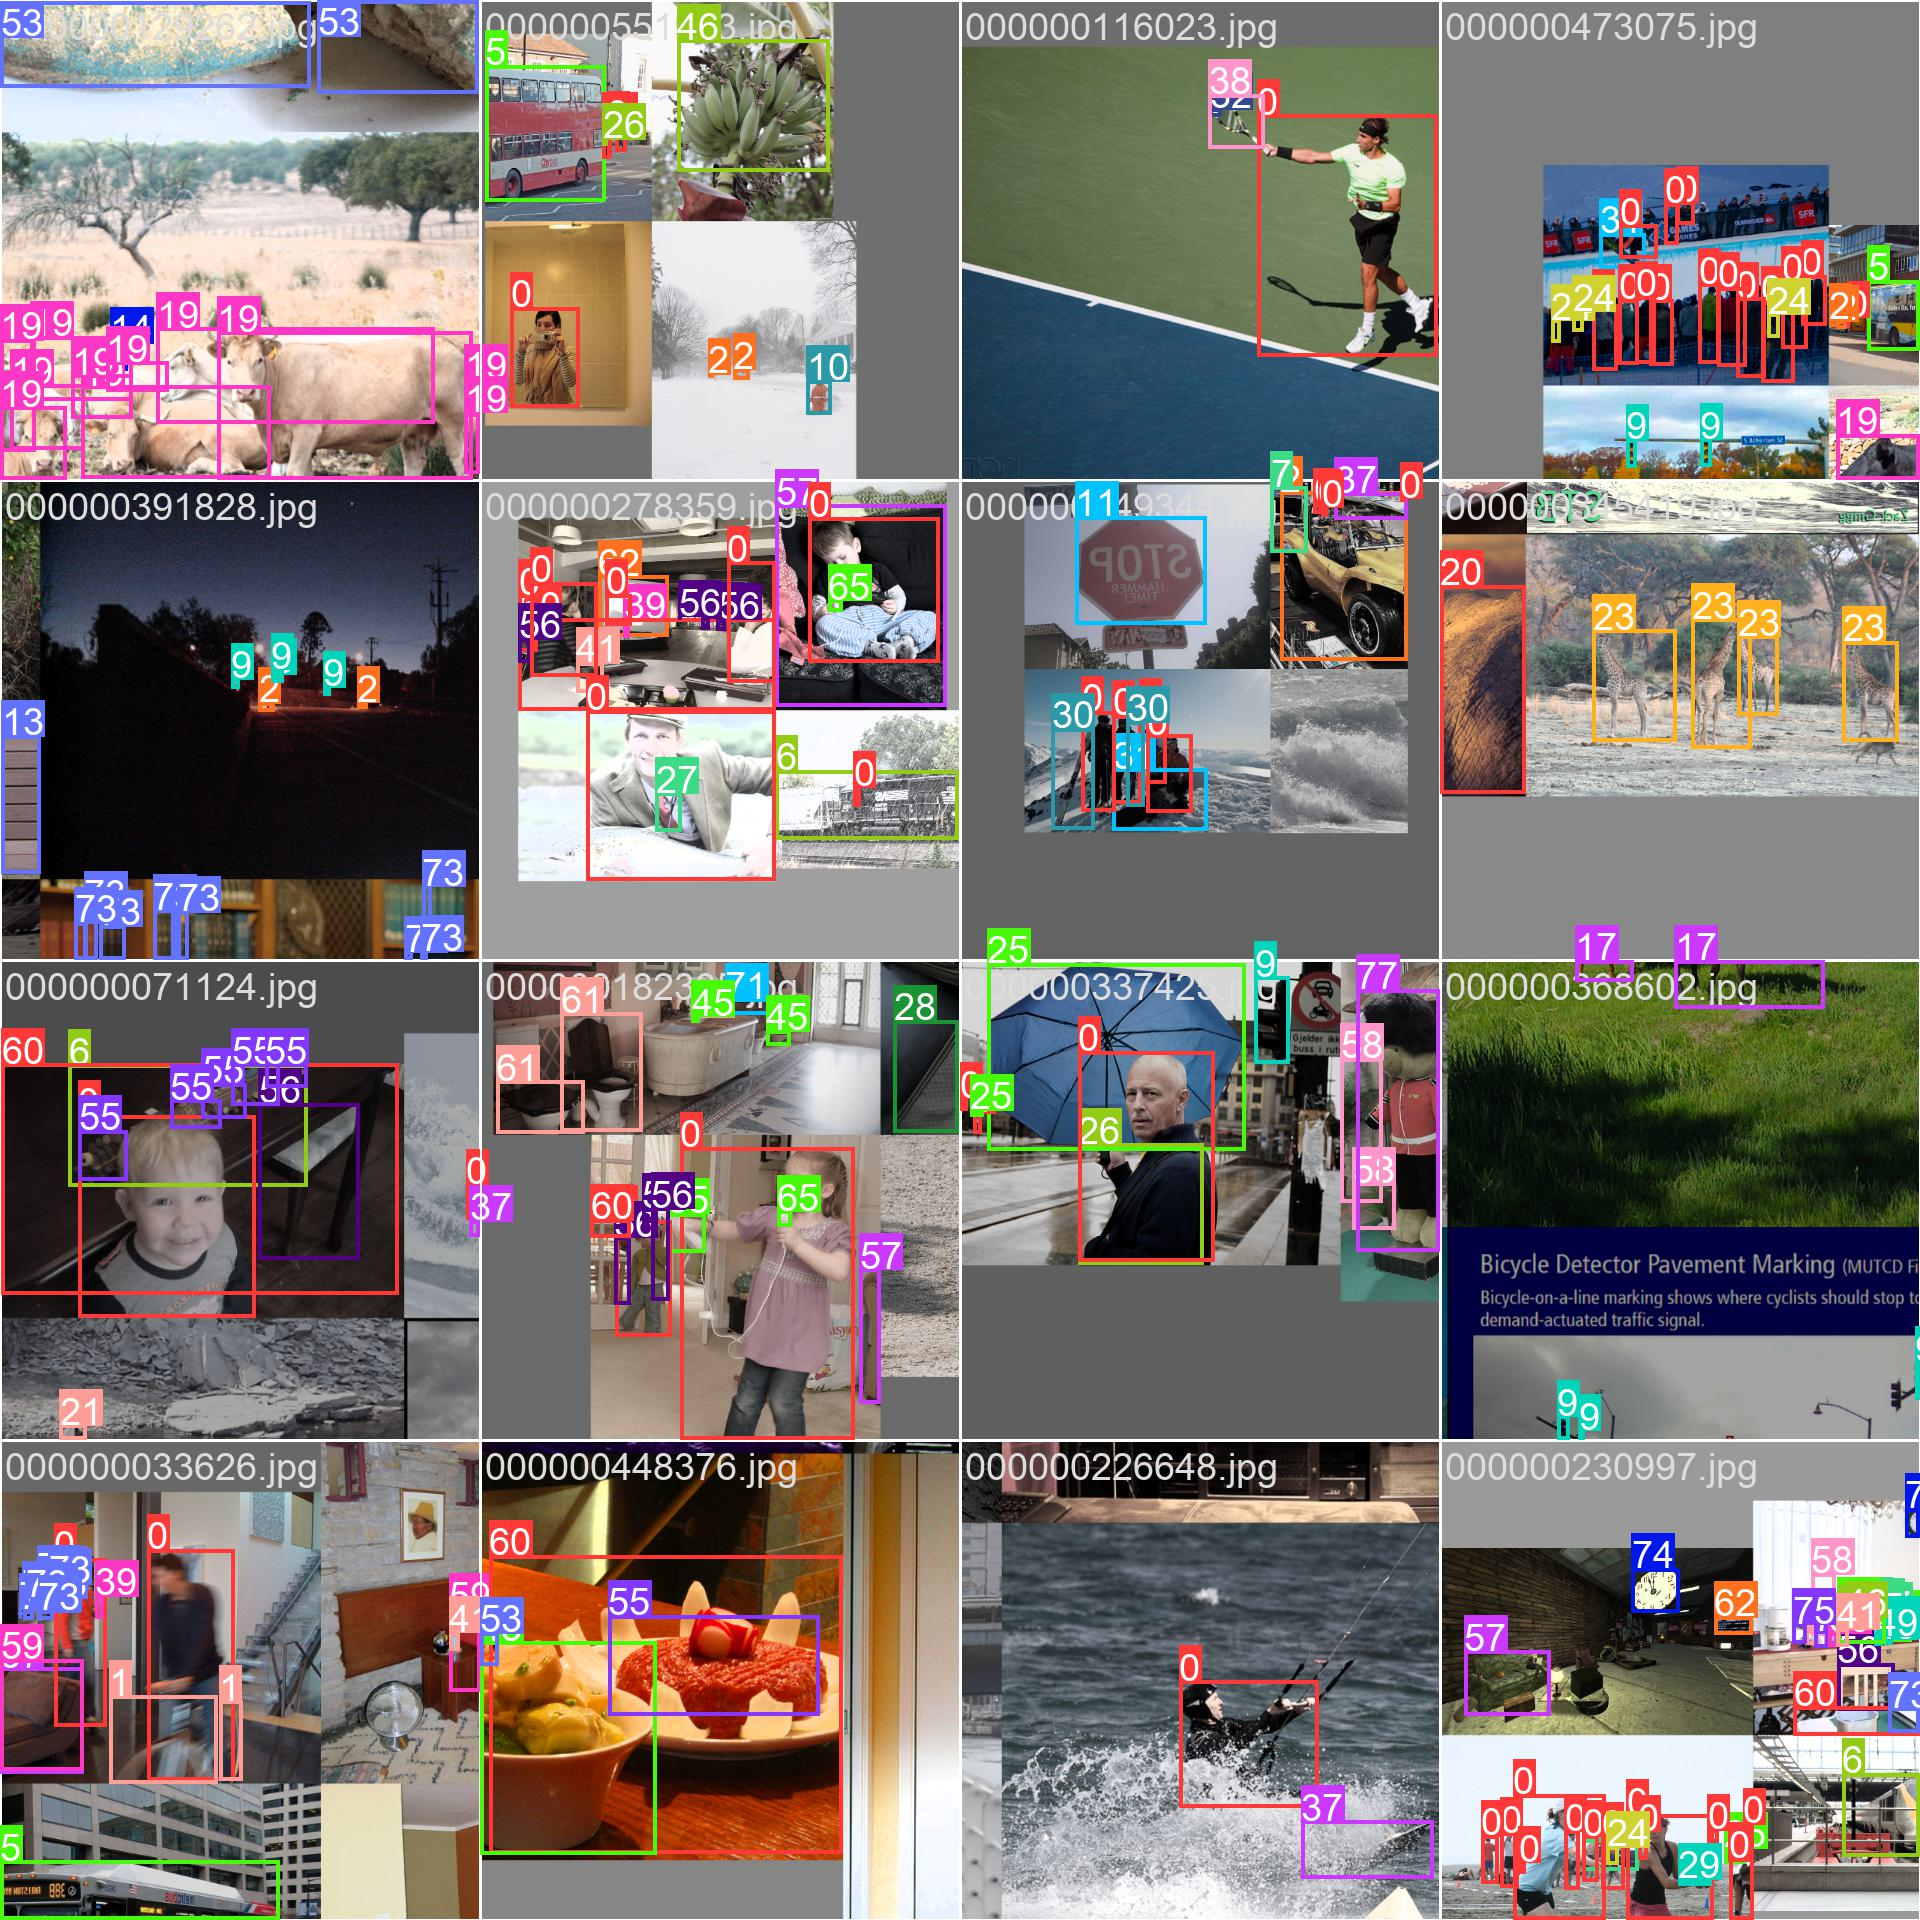
\includegraphics[width=0.8\linewidth]{img/annotations.jpg}
                \caption{Sample Images and Annotations}
                \label{fig:annotations}
            \end{figure}
    \subsection{Training Custom Datasets}
        Download my dataset from my preferred tool. In this example, we use a dataset from Roboflow which is a great annotation platform used by many developers and companies. The dataset is exported in COCO format. \\
        \vspace{3mm}
        In order to train YOLOv9 on my custom dataset, please create a new workflow from scratch. \\
        \vspace{3mm}
        Then I need 2 components:
        \begin{enumerate}
            \item A COCO dataset loader which loads dataset in COCO format and convert it to an Ikomia format
            \item The YOLOv9 training algorithm which loads dataset in Ikomia format
        \end{enumerate}
        \subsubsection{Supported Dataset Formats}
            \begin{figure}[H]
                \centering
                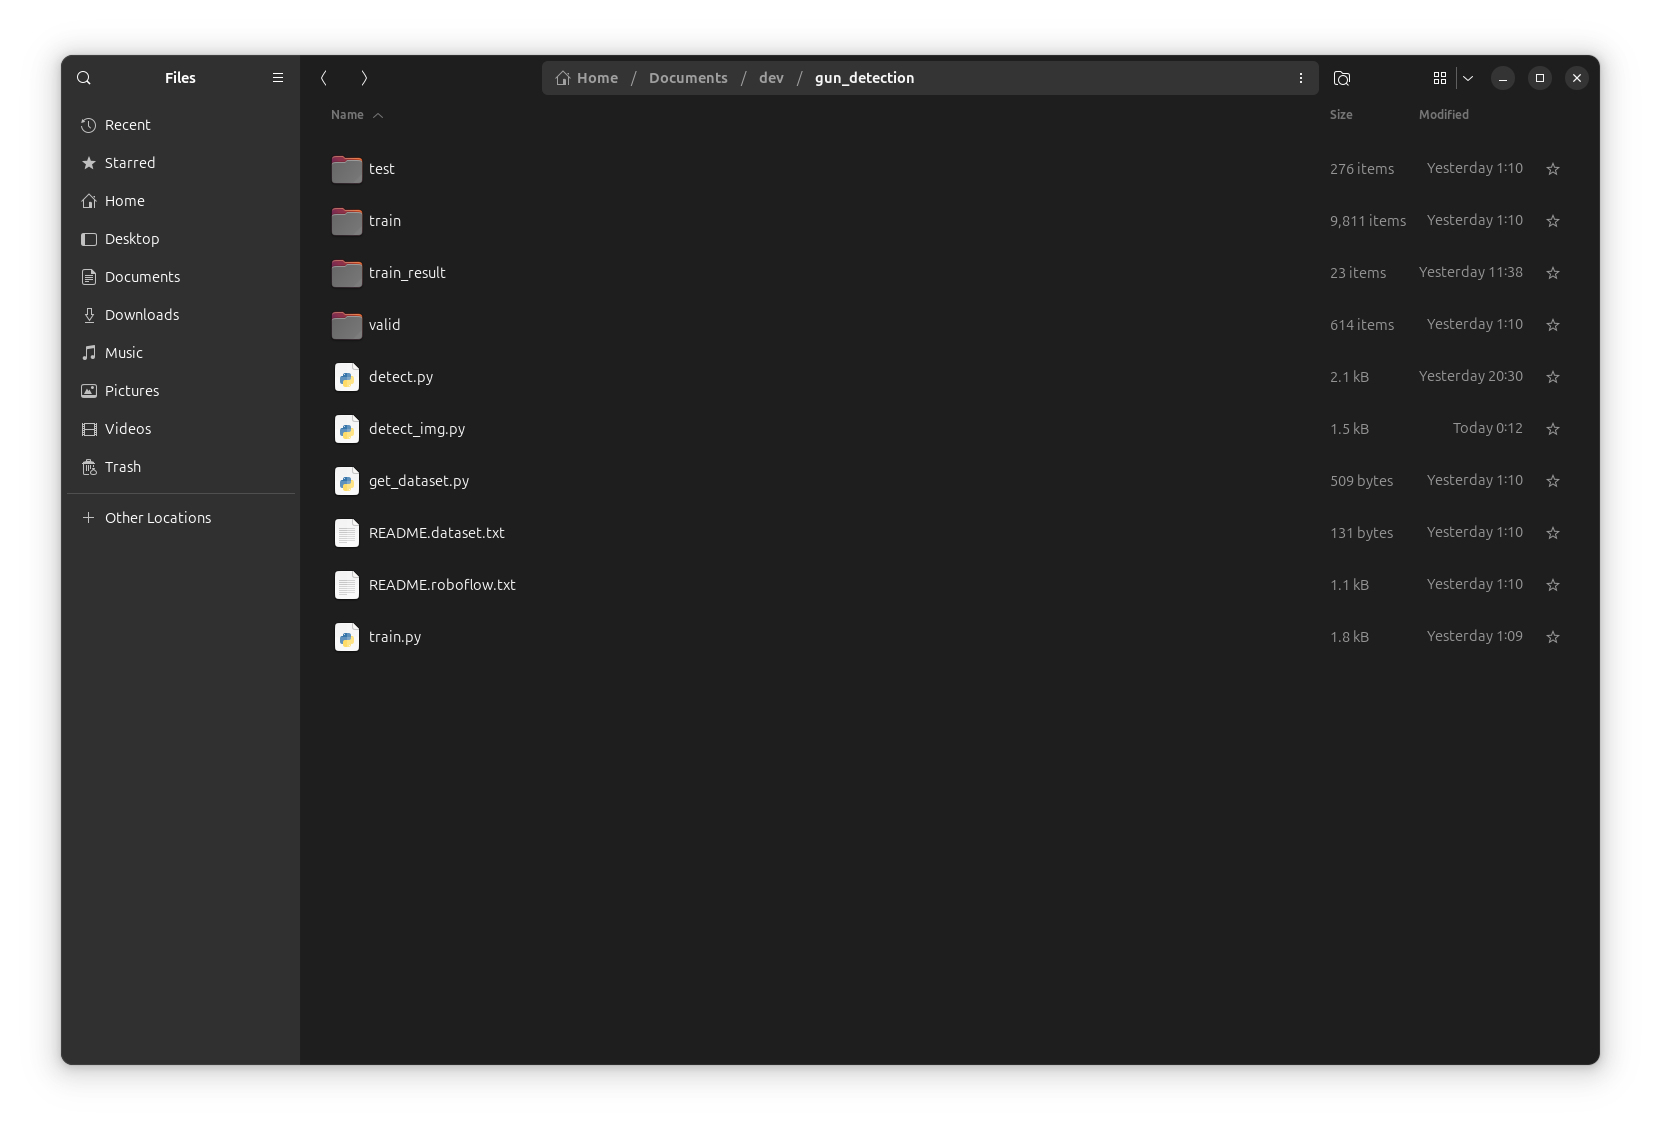
\includegraphics[width=0.8\linewidth]{img/folder_structure.png}
                \caption{COCO Dataset Structure}
                \label{fig:structure}
            \end{figure}
        \subsubsection{Performance on MS COCO Dataset}
            The performance of YOLOv9 on the \textbf{COCO dataset} exemplifies its significant advancements in real-time object detection, setting new benchmarks across various model sizes. Table \ref{tab:object-detector} presents a comprehensive comparison of state-of-the-art real-time object detectors, illustrating YOLOv9's superior efficiency and accuracy.
            \begin{table}[ht]
                \centering
                \small
                \begin{tabular}{| l | l | l | l | l | l |}
                    \hline
                    \rowcolor{lightgray} Model & Size (pixels) & mAP${^{val}_{50:95}}$ & mAP${^{val}_{50}}$ & params (M) & FLOPs (B) \\ \hline
                    YOLOv9t & 640 & 38.3 & 53.1 & 2.0 & 7.7 \\ \hline
                    YOLOv9s & 640 & 46.8 & 63.4 & 7.2 & 26.7 \\ \hline
                    YOLOv9m & 640 & 51.4 & 68.1 & 20.1 & 76.8 \\ \hline
                    YOLOv9c & 640 & 53.0 & 70.2 & 25.5 & 102.8 \\ \hline
                    YOLOv9e & 640 & 55.6 & 72.8 & 58.1 & 192.5 \\ \hline
                \end{tabular}
                \caption{Comparison of State-of-the-Art Real-Time Object Detectors}
                \label{tab:object-detector}
            \end{table}
            YOLOv9's iterations, ranging from the tiny \textbf{\textit{t}} variant to the extensive \textbf{\textit{e}} model, demonstrate improvements not only in accuracy (mAP metrics) but also in efficiency with a reduced number of parameters and computational needs (FLOPs). This table underscores YOLOv9's ability to deliver high precision while maintaining or reducing the computational overhead compared to prior versions and competing models. \\
            \vspace{3mm}
            Comparatively, YOLOv9 exhibits remarkable gains:
            \begin{itemize}
                \item \textbf{Lightweight Models:} YOLOv9s surpasses the YOLO MS-S in parameter efficiency and computational load while achieving an improvement of 0.4$\sim$0.6\% in AP.
                \item \textbf{Medium to Large Models:} YOLOv9m and YOLOv9e show notable advancements in balancing the trade-off between model complexity and detection performance, offering significant reductions in parameters and computations against the backdrop of improved accuracy.
            \end{itemize}
            The YOLOv9c model, in particular, highlights the effectiveness of the architecture's optimizations. It operates with 42\% fewer parameters and 21\% less computational demand than YOLOv7 AF, yet it achieves comparable accuracy, demonstrating YOLOv9's significant efficiency improvements. Furthermore, the YOLOv9e model sets a new standard for large models, with 15\% fewer parameters and 25\% less computational need than YOLOv8x, alongside a incremental 1.7\% improvement in AP. \\
            \vspace{3mm}
            These results showcase YOLOv9's strategic advancements in model design, emphasizing its enhanced efficiency without compromising on the precision essential for real-time object detection tasks. The model not only pushes the boundaries of performance metrics but also emphasizes the importance of computational efficiency, making it a pivotal development in the field of computer vision.
        \subsubsection{Start Training}
            In this work, we will have 4 steps to start training on our custom datasets:
            \begin{enumerate}
                \item \textbf{Step 1:} Create a workflow which will take your dataset as input and train a YOLOv9 model on it
                \item \textbf{Step 2:} First you need to convert the COCO format to IKOMIA format. Add an Ikomia dataset converter to your workflow.
                \item \textbf{Step 3:} Then, you want to train a YOLOv9 model. Add YOLOv9 training algorithm to your workflow
                \item \textbf{Step 4:} Execute your workflow. It automatically runs all your tasks sequentially.
            \end{enumerate}
            \begin{figure}[H]
                \centering
                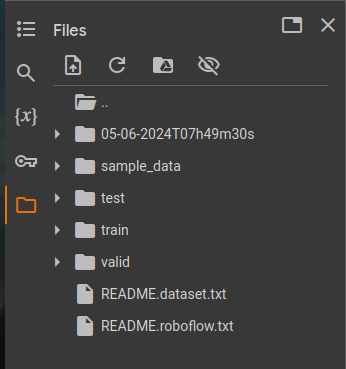
\includegraphics[width=0.8\linewidth]{img/project_tree.png}
                \caption{Project Tree on Colab environment}
                \label{fig:tree}
            \end{figure}
            Model will be trai
            After training finished, we will have an output like below:
            \begin{figure}[H]
                \centering
                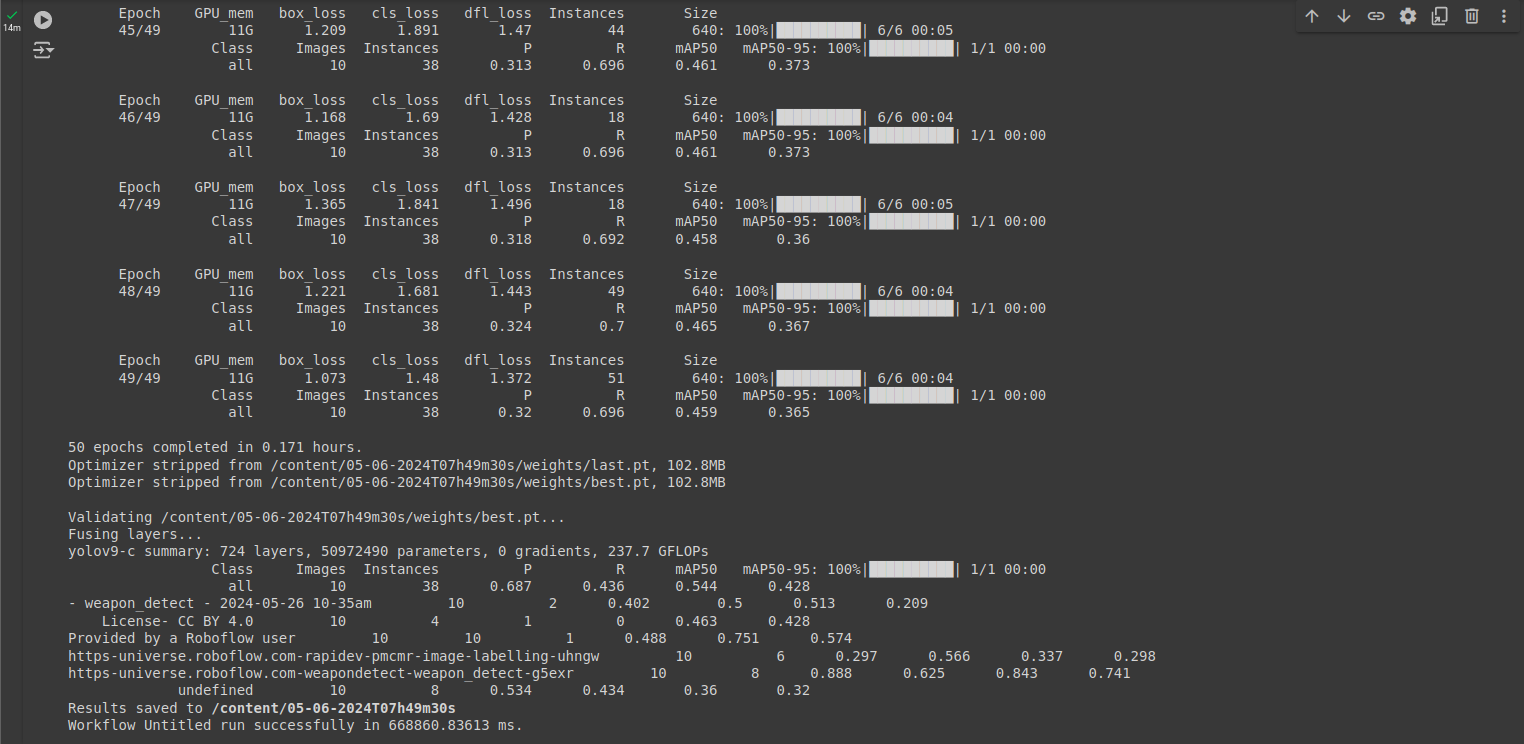
\includegraphics[width=0.8\linewidth]{img/train_result.png}
                \caption{COCO Dataset Training Result}
                \label{fig:train-result}
            \end{figure}
            Model will be trained with 20 epochs. We will do so using the GELAN-C architecture, one of the two architectures released as part of the YOLOv9 GitHub repository. GELAN-C is fast to train. GELAN-C inference times are fast, too. \\
            \vspace{3mm}
            With Google Colab environment, it will be trained with 50 epochs and with 8 batch\_size using 15GB GPU memory, so it just take 15 minutes to complete training process. 
            \begin{figure}[H]
                \centering
                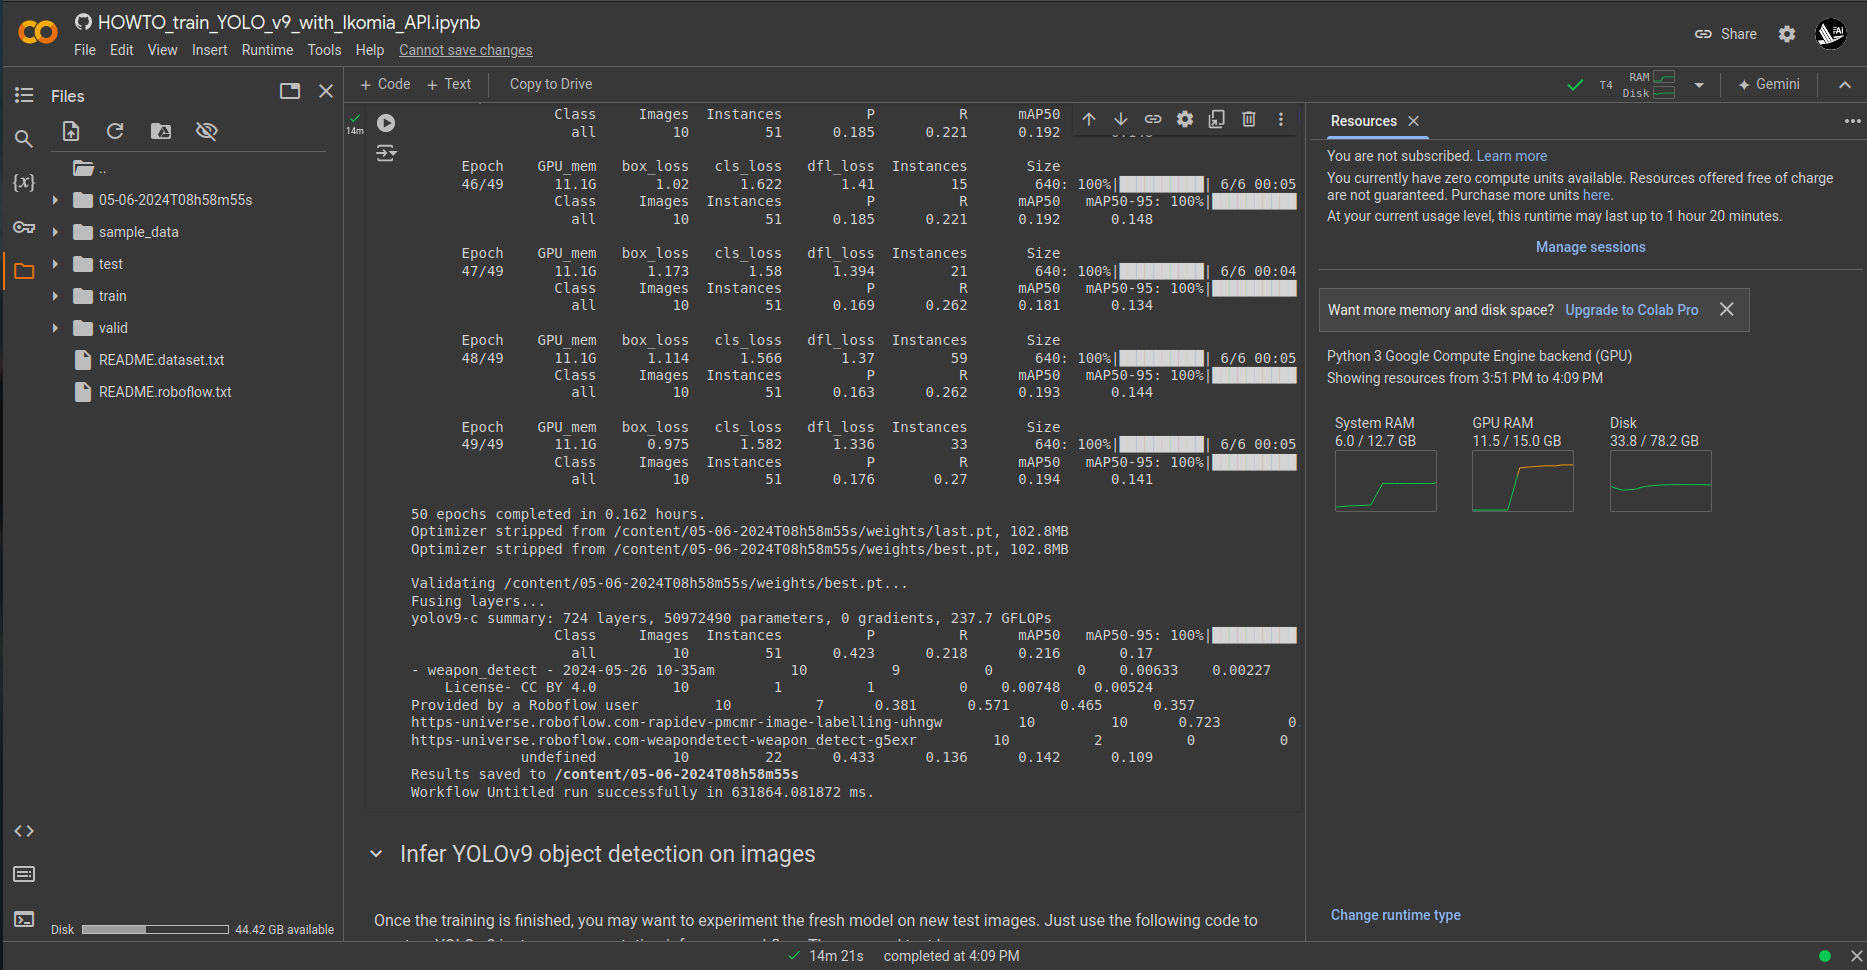
\includegraphics[width=0.8\linewidth]{img/colab_env.png}
                \caption{Google Colab Environment}
                \label{fig:colab-env}
            \end{figure}
            The training process for 20 epochs was completed in approximately 8 hours using an NVIDIA GeForce RTX 3060 12GB GPU. \\
            \vspace{3mm}
            \begin{figure}[H]
                \centering
                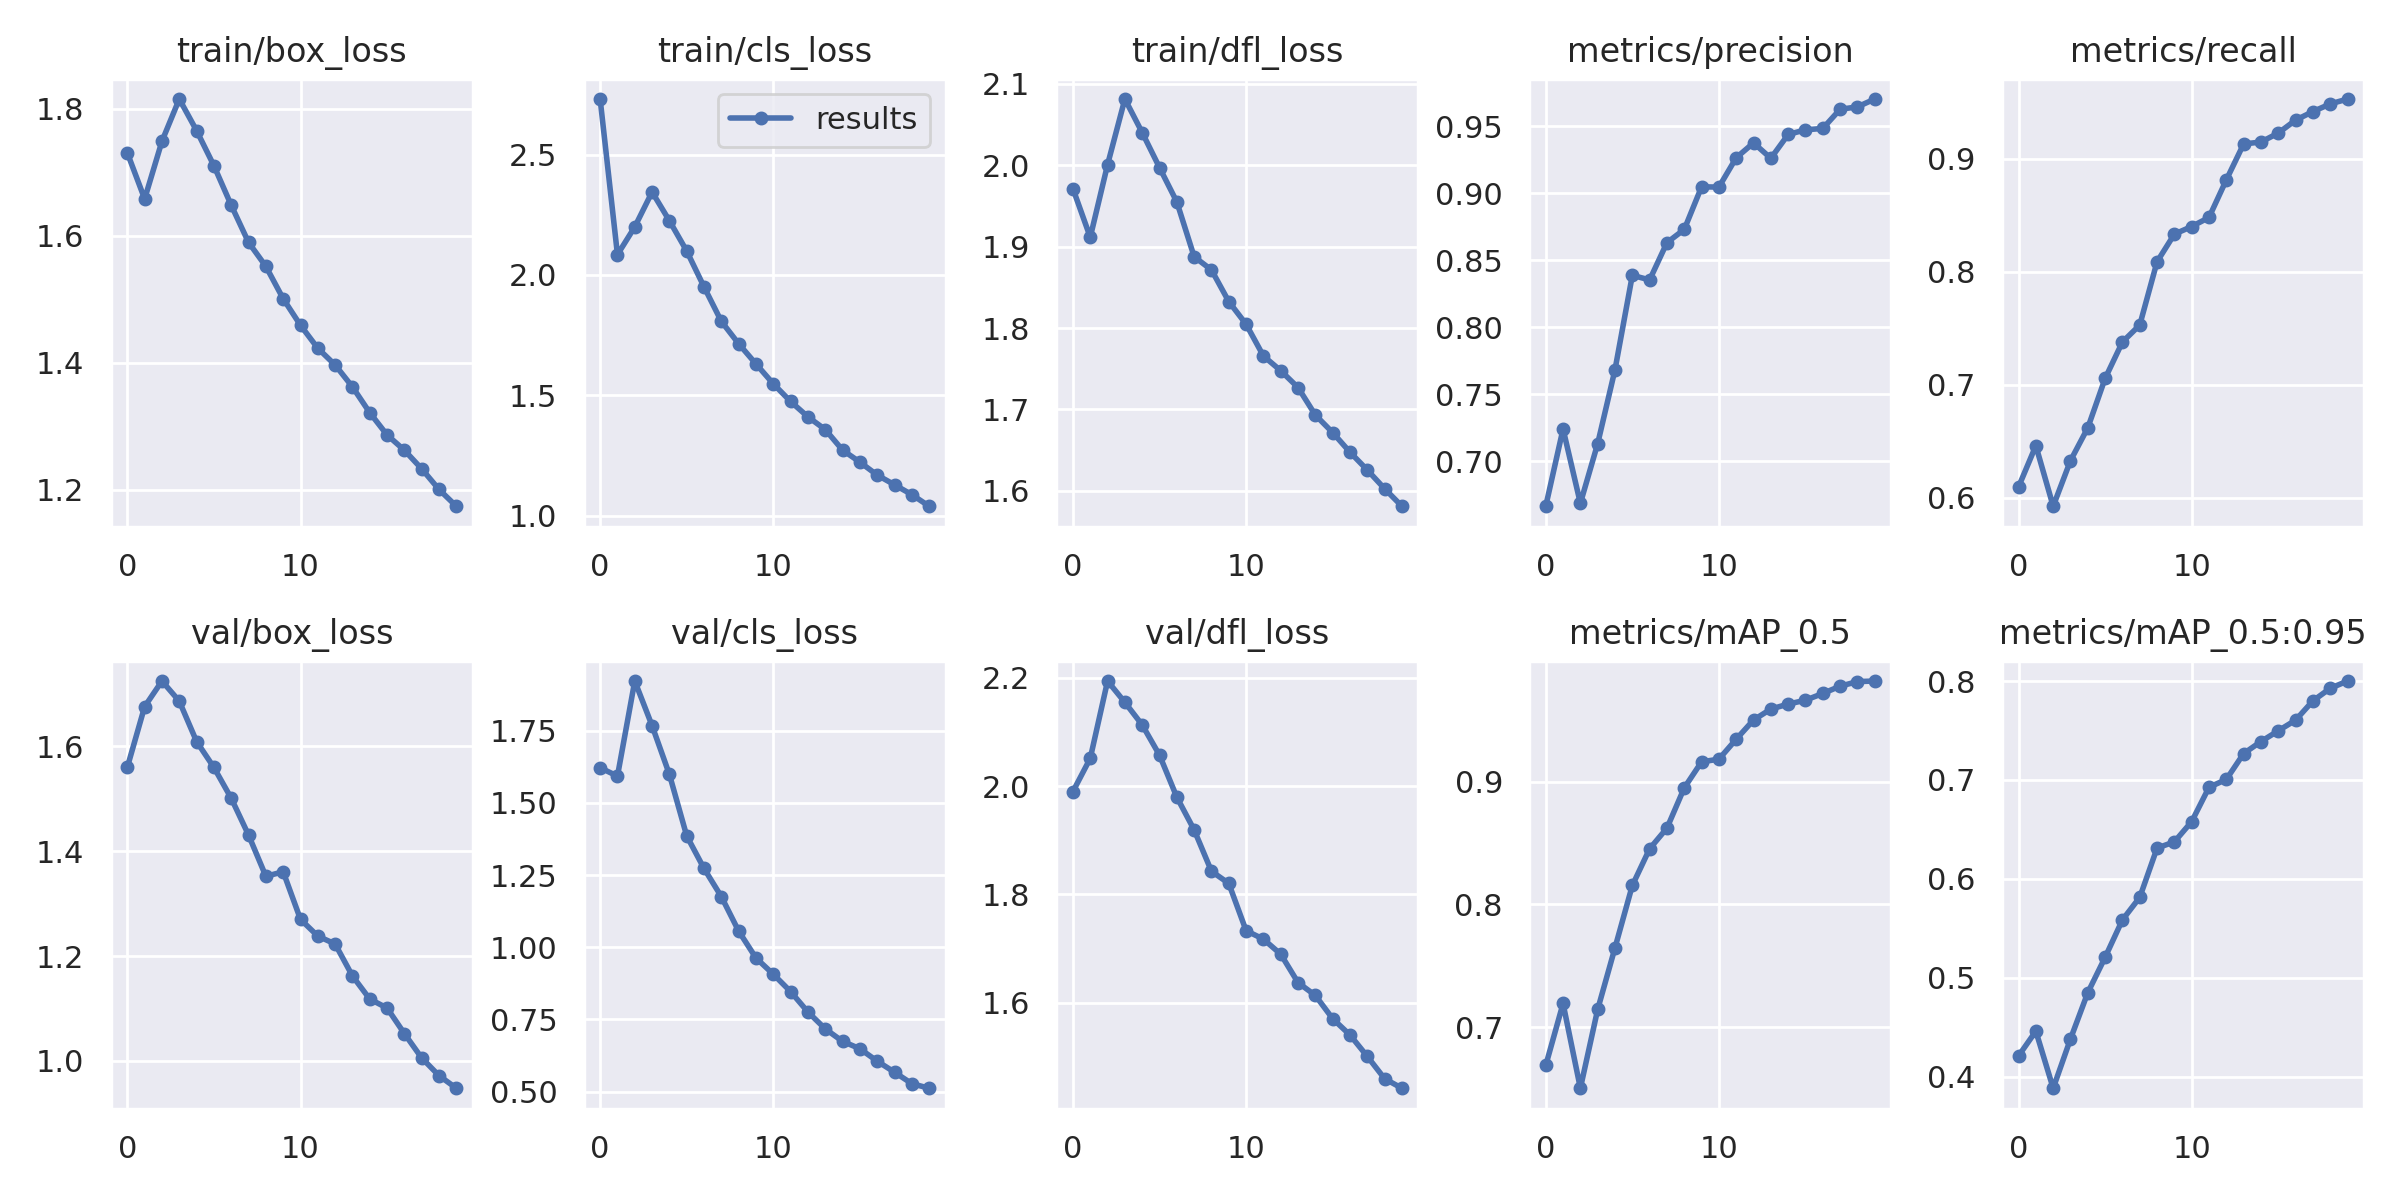
\includegraphics[width=0.8\linewidth]{img/results.png}
                \caption{COCO Dataset Training Graph}
                \label{fig:graph-result}
            \end{figure}
    \subsection{Infer YOLOv9 object detection on images}
        \begin{figure}[H]
            \centering
            \minipage{0.8\textwidth}
                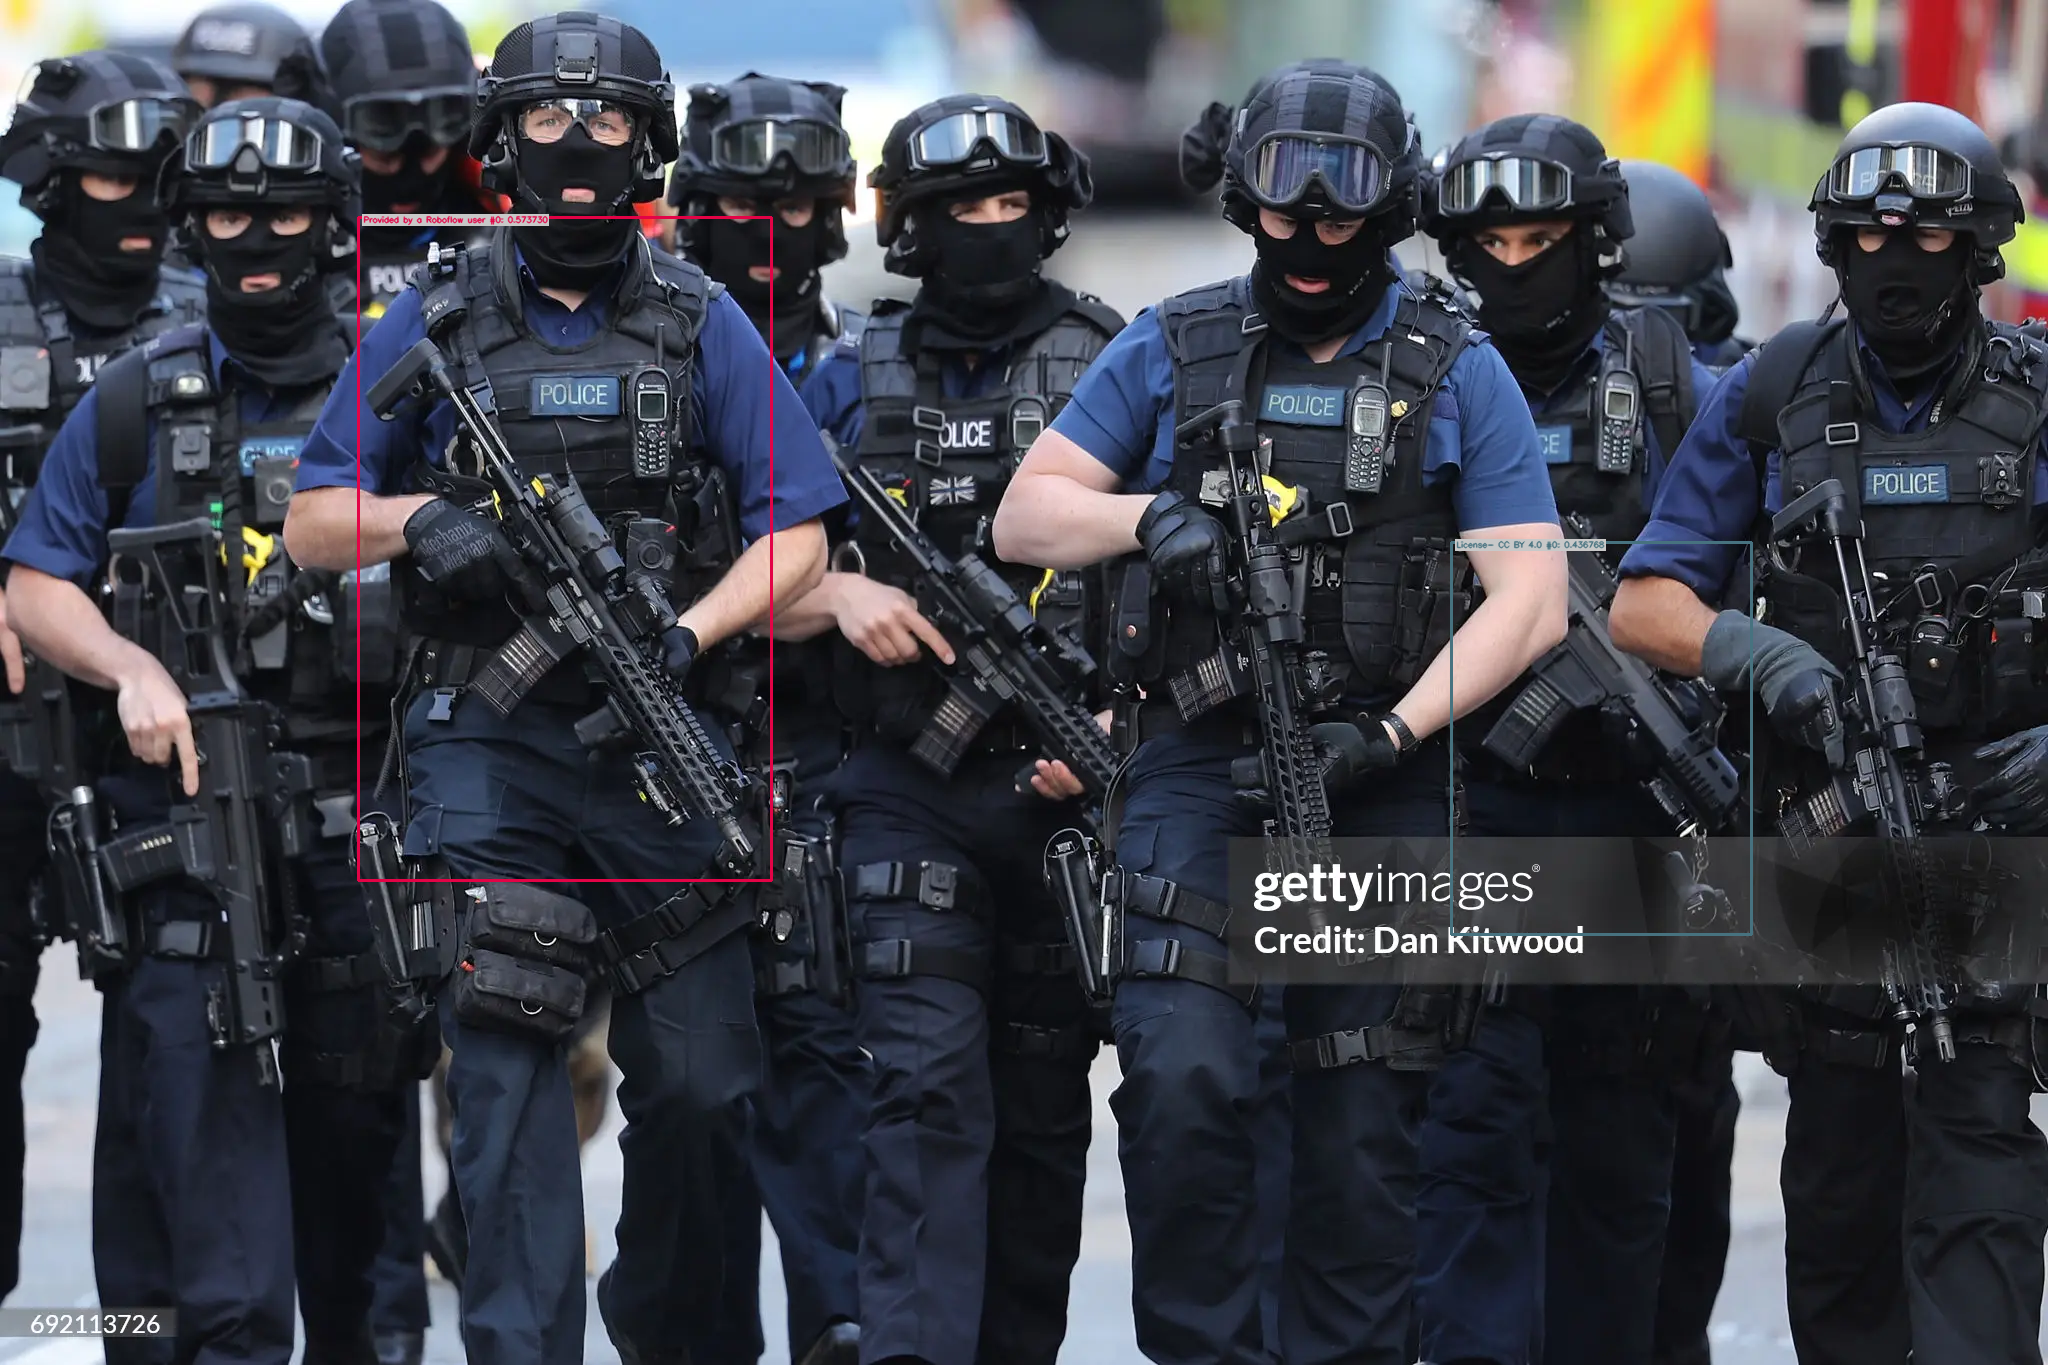
\includegraphics[width=0.8\linewidth]{img/gun_detect.png}
            \endminipage\hfill
            \minipage{0.8\textwidth}%
                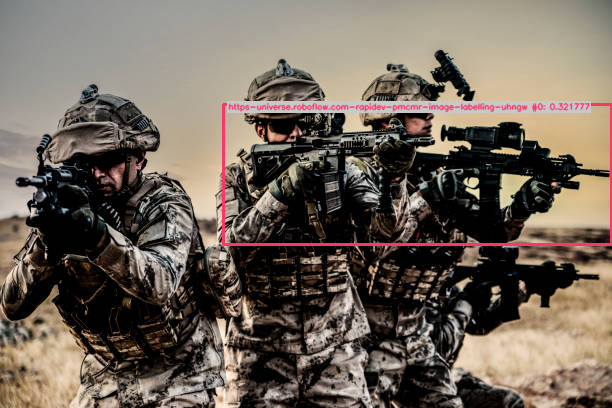
\includegraphics[width=0.8\linewidth]{img/gun_detect_result.png}
            \endminipage\hfill
            \caption{Gun Detect Image Result}
            \label{fig:image-result}
        \end{figure}
    \subsection{Infer YOLOv9 object detection on videos}
        \begin{figure}[H]
            \centering
            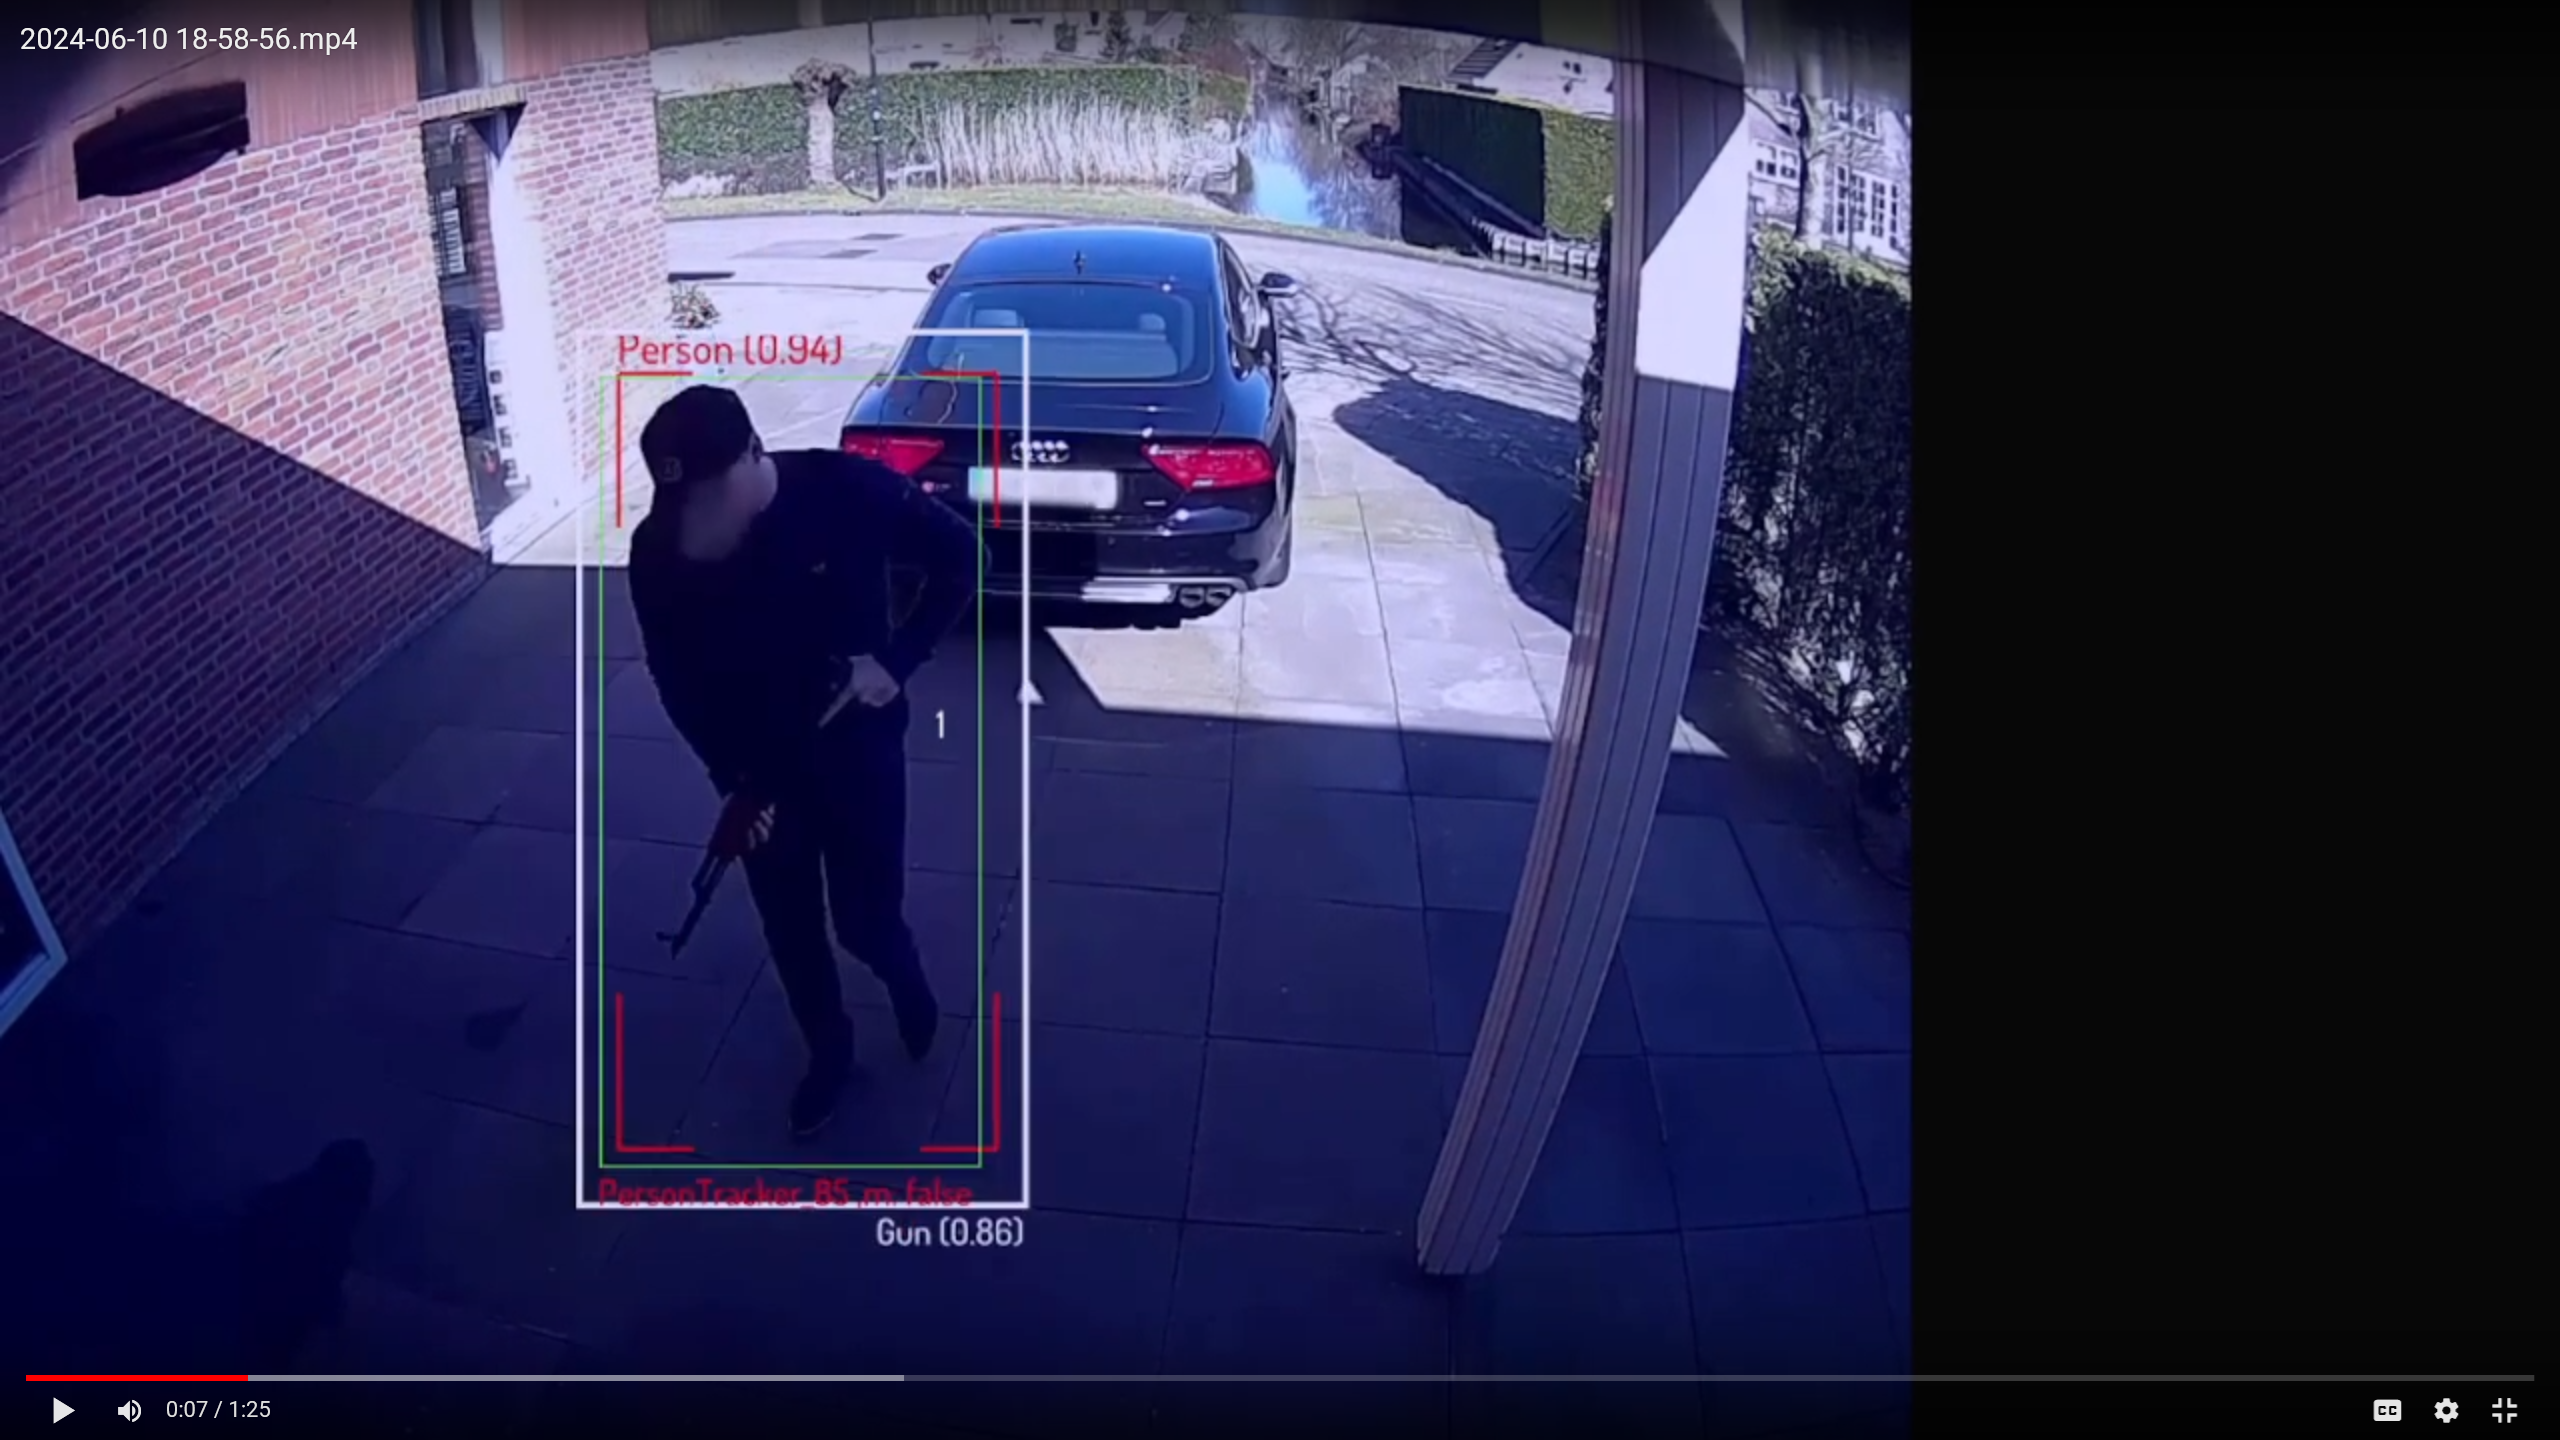
\includegraphics[width=0.8\linewidth]{img/result_data.png}
            \caption{Gun Detect Video Result}
            \label{fig:video-result}
        \end{figure}